\documentclass{article}
\usepackage[utf8]{inputenc}
\usepackage{hyperref}
\usepackage{listings}
\usepackage{color}
\usepackage{makecell}
\usepackage{graphicx}
\usepackage{titlepic}


\definecolor{dkgreen}{rgb}{0,0.6,0}
\definecolor{gray}{rgb}{0.5,0.5,0.5}
\definecolor{mauve}{rgb}{0.58,0,0.82}

\lstset{frame=tb,
  language=sql,
  aboveskip=3mm,
  belowskip=3mm,
  showstringspaces=false,
  columns=flexible,
  basicstyle={\small\ttfamily},
  numbers=none,
  numberstyle=\tiny\color{gray},
  keywordstyle=\color{blue},
  commentstyle=\color{dkgreen},
  stringstyle=\color{mauve},
  breaklines=true,
  breakatwhitespace=true,
  tabsize=3
}

\title{Modul 346 LB2}
\titlepic{
\includegraphics[width=\textwidth]{images/titleimage.png}}
\author{Maurice Däppen, Mika Hannappel und Patrick Aeschlimann}
\date{December 2022/Januar 2023}

\begin{document}

\maketitle

{\clearpage}


\tableofcontents

{\clearpage}

\section{Einleitung}

Mithilfe dieses Dokumentes dukmentieren wir unsere 4 Workshops der LB2 vom Modul 346 welche laut LBV 70 Prozent der Modulnote ausmacht. Von den Workshops wurden uns 2 Vorgegeben und 2 durften wir frei wählen. Vorgegeben wurde uns die beiden AWS-Services EC2 und RDS. Selbst ausgewählt haben wir die AWS-Services S3 und Amazon ECS. Beim EC2 Service haben wir uns dazu entschieden einen Minecraft Server, ein Pi-Hole und einen VPN einzurichten. Mit RDS müssen wir eine Datenbank mit 2 Tabellen erstellen, mit S3 wollen wir eine NextCloud aufsetzten und mit ECS möchten wir eine kleine Wordpress-Seite hosten. 
\newline
\newline
Alle Workshops werden mit AWS durchgeführrt. Dafür verfügen alle 3 Lernenden über einen Account welchen uns Zugriff auf das AWS Learner Lab gibt. Pro Person haben wir in diesem Learner Lab 100 Dollar zu verfügung. In unserem Fall haben wir uns dazu entschiden nur einen dieser Accounts für unser fertiges Projekt zu nutzen damit wir alles zusammen haben was uns auch in den Modulunterlagen empfohlen wurde. Damit jedoch auch jeder in der Gruppe Zugriff auf diesen Account hat, haben wir ein Dummy Passwort für den Account von Maurice erstellt und die Login Daten geteilt. Mit den folgenden Logindaten kann man sich in diesen Account unter https://awsacademy.instructure.com/login/canvas einloggen:
\newline
\newline
E-Mail: mda133769@iet-gibb.ch
\newline
Passwort: sml12345
\newline
\newline
Viel Spass beim Lesen...



{\clearpage}

\section{EC2}


\subsection{Minecraft Server}

\begin{center}

\begin{tabular}{|l|l|}
\hline
\textbf{Key} & \textbf{Value} \\ \hline
Name des Webservers & MinecraftServer \\ \hline
Offene Ports von aussen & 22, 25565 \\ \hline
Public Netzwerk, inkl. Gateway und Route & Ja \\ \hline
User & ec2-user \\ \hline
Public Key & - \\ \hline
Software & Mincecraft Server \\ \hline
Region & us-east-1 \\ \hline
AMI & \makecell{Amazon Linux \\ (ami-0574da719dca65348)} \\ \hline
\end{tabular}

\end{center}

\vspace{10pt}

\noindent Wir haben unseren Minecraft Server Mithilfe eines Terraform-Skrites erstellt. Dafür haben wir das untenstehende Terraform Skript verwendet. In diesem Terraform Skript erstellen wir eine Sicherheitsgruppe names "minecraft" welche die TCP Ports 22 und 25565 von aussen für alle öffnet und von innen alle Ports für alle Protokolle öfnnet. Danach erstellen wir unseren Server mit dem Namen "minecraft" und wählen das AMI und die Instance Grösse aus. Zudem adden wir die oben erstelle Sicherheitsgruppe und unser Cloud-Init Skript welches nach der erstellung der Instance ausgeführt wird.

\vspace{30pt}

\begin{lstlisting}[caption=Terraform Script für Minecraft Server]
terraform {
  required_providers {
    aws = {
      source  = "hashicorp/aws"
      version = "~> 4.16"
    }
  }

  required_version = ">= 1.2.0"
}

provider "aws" {
  region  = "us-east-1"
}

data "template_file" "user_data" {
  template = file("./cloud-init.yaml")
}

resource "aws_security_group" "minecraft" {
  name        = "minecraft"
  description = "Security group for Minecraft server"

  ingress {
    protocol    = "tcp"
    from_port   = 25565
    to_port     = 25565
    cidr_blocks = ["0.0.0.0/0"]
  }
  
  ingress {
    protocol    = "tcp"
    from_port   = 22
    to_port     = 22
    cidr_blocks = ["0.0.0.0/0"]
  }
  egress {
    protocol    = "-1"
    from_port   = 0
    to_port     = 0
    cidr_blocks = ["0.0.0.0/0"]
  }
}

resource "aws_instance" "app_server" {
  ami           = "ami-0b5eea76982371e91"
  instance_type = "t2.small"

  vpc_security_group_ids = [aws_security_group.minecraft.id]
  
  user_data = data.template_file.user_data.rendered

  tags = {
    Name = "MinecraftServer"
  }
}
\end{lstlisting}

\vspace{20pt}

\noindent Danach haben wir den Server noch mit einem Cloud-Init Skript konfiguriert. In dem Cloud-Init Skript haben wir folgende Befehle ausgeführt:

\begin{itemize}

\item \texttt{sudo rpm --import https://yum.corretto.aws/corretto.key}: \\ 
Dieser Befehl importiert den GPG-Schlüssel für das Amazon Corretto-Paketrepository. Der GPG-Schlüssel wird verwendet, um die Echtheit und Integrität der heruntergeladenen Pakete zu überprüfen.

\item \texttt{sudo curl -L -o /etc/yum.repos.d/\\corretto.repo https://yum.corretto.aws/corretto.repo}: \\ 
Dieser Befehl lädt eine Konfigurationsdatei für das Amazon Corretto-Paketrepository herunter und speichert sie im Verzeichnis /etc/yum.repos.d/ auf dem System.


\item \texttt{sudo yum install -y java-17-amazon-corretto-devel}: \\ 
Dieser Befehl installiert das Amazon Corretto 17-Entwicklungskit (JDK) auf dem System.

\item \texttt{sudo adduser minecraft}: \\ 
Dieser Befehl fügt einen Minecraft-Benutzer hinzu.

\item \texttt{sudo su}: \\ 
Mit diesem Befehl wird eine Superuser-Sitzung gestartet.

\item \texttt{mkdir /opt/minecraft/}: \\ 
Dieser Befehl erstellt das Verzeichnis /opt/minecraft/.

\item \texttt{mkdir /opt/minecraft/server/}: \\ 
Dieser Befehl erstellt das Verzeichnis /opt/minecraft/server/.

\item \texttt{cd /opt/minecraft/server}: \\ 
Mit diesem Befehl wechselt man in das Verzeichnis /opt/minecraft/server/.

\item \texttt{wget https://launcher.mojang.com/v1/objects/\\c8f83c5655308435b3dcf03c06d9fe8740a77469/server.jar}: \\ 
Mit diesem Befehl wird die Datei server.jar vom Minecraft-Server heruntergeladen und im aktuellen Verzeichnis gespeichert.

\item \texttt{sudo chown -R minecraft:minecraft /opt/minecraft/}: \\ 
Mit diesem Befehlt wechselt man den Eigentümer vom oben zu sehenden Verzeichniss zum User Minecraft. 

\item \texttt{java -Xmx1024M -Xms1024M -jar server.jar nogui}: \\ 
Mit diesem Befehl versuchen wir den Minecraft Server zu starten. Die wird jedoch nicht funktionieren da wir der EULA noch nicht zugestummen haben. Diese wir somit nun erstellt und im selben Verzeichniss abgelegt.

\item \texttt{sudo sed -i 's/eula=false/eula=true/' eula.txt}: \\ 
Mit diesem Befhel ersetzen "eula=false" zu "eula=true" im File eula.txt. Die bewirkt dass die ELUA nun angenommen wure.

\vspace{30pt}

Jetzt ist der Server bereit zu starten. Dies können mit folgendem Befehlt erreichen: "sudo java -Xmx1024M -Xms1024M -jar server.jar nogui". Man benötigt jetzt nur noch einen Minecraft-Client und einen Minecraft Account und man kann auf dem Server spielen. 
Mit der IP welche man in AWS auf der Instance nachschauen kann, kann man dem Server betreten.
\end{itemize}
\clearpage


\subsection{Pihole}

\begin{center}

\begin{tabular}{|l|l|}
\hline
\textbf{Key} & \textbf{Value} \\ \hline
Name des Webservers & PiHoleServer \\ \hline
Offene Ports von aussen & 22, 80, 443 \\ \hline
Public Netzwerk, inkl. Gateway und Route & Ja \\ \hline
User & ubuntu \\ \hline
Public Key & pihole key \\ \hline
Software & Pi-Hole \\ \hline
Region & us-east-1 \\ \hline
AMI & \makecell{Ubuntu  \\ (ami-0574da719dca65348)} \\ \hline
\end{tabular}

\end{center}

\vspace{10pt}

\noindent Auch den Server für das Pi-Hole haben wir mit der Hilfe eines Terraform Skriptes ausgesetzt. Dafür haben wir das untenstehende Skript verwendet. Auch dieses mal haben wir wieder eine Sicherheitsgruppe erstellt. Diese Sicherheitsgruppe öffnet die Ports 22, 80 und 443 von aussen für alle. Unn auch wieder von innen werden alle Ports für alle Protokolle geöffnet. Danach erstellen wir wieder unsere Instance, wählen das Amazon Machine Image und die grösse der Instance. Zudem fügen wir unser Keypair und die Sicherheitsgruppe hinzu. Zum Schluss adden wir noch das Cloud-Init Skript welches nach dem die Instance ferit aufgesetzt ist ausgeführt wird.

\vspace{30pt}

\begin{lstlisting}[caption=Terraform Script für Pi-hole Server]
terraform {
  required_providers {
    aws = {
      source  = "hashicorp/aws"
      version = "~> 4.16"
    }
  }

  required_version = ">= 1.2.0"
}

provider "aws" {
  region  = "us-east-1"
}

data "template_file" "user_data" {
  template = file("./cloud-init.yaml")
}

resource "aws_security_group" "pi_hole" {
  name        = "pi_hole"
  description = "Security group for Pi-Hole server"

  ingress {
    protocol    = "tcp"
    from_port   = 80
    to_port     = 80
    cidr_blocks = ["0.0.0.0/0"]
  }
  
  ingress {
    protocol    = "tcp"
    from_port   = 443
    to_port     = 443
    cidr_blocks = ["0.0.0.0/0"]
  }
  
  ingress {
    protocol    = "tcp"
    from_port   = 22
    to_port     = 22
    cidr_blocks = ["0.0.0.0/0"]
  }
  egress {
    protocol    = "-1"
    from_port   = 0
    to_port     = 0
    cidr_blocks = ["0.0.0.0/0"]
  }
}

resource "aws_instance" "app_server" {
  ami           = "ami-0574da719dca65348"
  instance_type = "t2.medium"
  key_name      = "pihole key"
  vpc_security_group_ids = [aws_security_group.pi_hole.id]
  
  user_data = data.template_file.user_data.rendered

  tags = {
    Name = "PiHoleServer"
  }
}
\end{lstlisting}

\clearpage

\noindent Die folgenden Befele werden im Cloud-Init Skript ausgeführt und bringen die Ubuntu Instance auf den neusten stand und führen die ersten Schritte für die Pi-Hole Einrichtung aus.

\begin{itemize}
\item \texttt{sudo apt update}: \\
Aktualisiert die Liste der verfügbaren Pakete und ihrer Versionen, die von den Paketquellen im System verwendet werden.

\item \texttt{sudo apt upgrade -y}: \\
Aktualisiert installierte Pakete auf ihre neuesten verfügbaren Versionen. Die Option \texttt{-y} sagt dem System, alle Abhängigkeitsfragen automatisch mit \texttt{"Ja"} zu beantworten.

\item \texttt{sudo hostnamectl: \\
Set-hostname AWS\_PiHole} ändert den Hostnamen des Systems in \\
\texttt{"AWS\_PiHole"}.
\end{itemize}

\noindent Von diesem Punkt an konnte wir leider nicht mehr mit einem Skript arbeiten da für die Pi-Hole Instalation einige Installer mit "Pop-Ups" auftreten bei welchen man manuell bestätigen muss und wir leider keinen Weg fanden dies zu umgehen. Deshalb wrden die folgenden Befehle manuell auf der Instance ausgeführt.

\begin{itemize}
    \item \texttt{sudo curl -sSL https://install.pi-hole.net | bash}: \\
Lädt ein Skript von der angegebenen URL herunter und führt es aus. Dieses Skript installiert Pi-hole auf dem System.

\item \texttt{pihole -a -p}: \\
Startet den Pi-hole-Assistenten und führt ihn im \texttt{"privaten"} Modus aus. Im \texttt{"privaten"} Modus werden keine Informationen über die Konfiguration an den Pi-hole-Server gesendet.
\end{itemize}

\noindent Mit der IP, weclhe man in AWS auf der Instance nachschauen kann, kann man nun über einen Browser auf das PI-Hole Admin Dashboard zugreiffen. Um sich einzuloggen verwendet man als Password "sml12345".

\clearpage

\subsection{VPN}

\begin{center}

\begin{tabular}{|l|l|}
\hline
\textbf{Key} & \textbf{Value} \\ \hline
Name des Webservers & OpenVpnServer \\ \hline
Offene Ports von aussen & 22, 80, 443, 1194 \\ \hline
Public Netzwerk, inkl. Gateway und Route & Ja \\ \hline
User & ubuntu \\ \hline
Public Key & vpn \\ \hline
Software & Open Vpn \\ \hline
Region & us-east-1 \\ \hline
AMI & \makecell{Ubuntu  \\ (ami-0574da719dca65348)} \\ \hline
\end{tabular}

\end{center}

\vspace{10pt}

\noindent Wie auch schon für die anderen EC2 Instances haben wir auch für den VPN ein Terraform-Skript verwendet. Als erstes erstellen wir wieder eine Sicherheitsgruppe mit dem Namen "vpn" welche von aussen die Ports 22, 80, 443 und 1194 öffnet. Von Innen darf natürlich auf alles zugegriffen werden. Danach erstellen wir die eigentliche Instance. Für diese verwenden wir wie beim PiHole ein Ubuntu Image mit der Grösse t2.micro. Ausserdem weisen wir noch die oben erstelle Sicherheitsgruppe zu, ein keypair welches wir bereits in aws erstellt haben und das Cloud-Init Skript welches die Maschine aktualisiert.

\vspace{30pt}

\begin{lstlisting}[caption=Terraform Script für VPN Server]
terraform {
  required_providers {
    aws = {
      source  = "hashicorp/aws"
      version = "~> 4.16"
    }
  }

  required_version = ">= 1.2.0"
}

provider "aws" {
  region  = "us-east-1"
}

data "template_file" "user_data" {
  template = file("./cloud-init.yaml")
}

resource "aws_security_group" "vpn" {
  name        = "vpn"
  description = "Security group for OpenVpn server"

  ingress {
    protocol    = "tcp"
    from_port   = 80
    to_port     = 80
    cidr_blocks = ["0.0.0.0/0"]
  }
  
  ingress {
    protocol    = "tcp"
    from_port   = 443
    to_port     = 443
    cidr_blocks = ["0.0.0.0/0"]
  }
  
  ingress {
    protocol    = "tcp"
    from_port   = 22
    to_port     = 22
    cidr_blocks = ["0.0.0.0/0"]
  }
  
  ingress {
    protocol    = "tcp"
    from_port   = 1194
    to_port     = 1194
    cidr_blocks = ["0.0.0.0/0"]
  }
  
  ingress {
    protocol    = "udp"
    from_port   = 1194
    to_port     = 1194
    cidr_blocks = ["0.0.0.0/0"]
  }
  egress {
    protocol    = "-1"
    from_port   = 0
    to_port     = 0
    cidr_blocks = ["0.0.0.0/0"]
  }
}

resource "aws_instance" "app_server" {
  ami           = "ami-0574da719dca65348"
  instance_type = "t2.micro"
  key_name      = "vpn"
  vpc_security_group_ids = [aws_security_group.vpn.id]
  
  user_data = data.template_file.user_data.rendered

  tags = {
    Name = "OpenVpnServer"
  }
}
\end{lstlisting}


\noindent Die folgenden Befele werden im Cloud-Init Skript, welches wir oben geaddet haben, ausgeführt und bringen die Ubuntu Instance auf den neusten stand..

\begin{itemize}
\item \texttt{sudo apt update}: \\
Aktualisiert die Liste der verfügbaren Pakete und ihrer Versionen, die von den Paketquellen im System verwendet werden.
\end{itemize}

\noindent Ansonsten haben wir leider nichts ins Cloud-Init Skript schreiben können da wir die Installer Pop-Ups nicht automatisieren können. Die folgenden Befehle haben wir manuel auf der EC2 Instance ausgeführt:

\begin{itemize}
\item \texttt{sudo apt update}: \\
Aktualisiert die Liste der verfügbaren Pakete und ihrer Versionen, die von den Paketquellen im System verwendet werden.

\item \texttt{sudo apt upgrade -y}: \\
Dieser Befehl aktualisiert die Liste der verfügbaren Pakete und führt ein Upgrade der bereits installierten Pakete durch. Der Parameter -y bestätigt automatisch alle Abfragen während des Upgrades.

\item \texttt{wget https://raw.githubusercontent.com/angristan/openvpn-install/master/openvpn-install.sh}: \\
Mit diesem Befehl wird eine Kopie der angegebenen Datei von GitHub heruntergeladen.

\item \texttt{chmod +x openvpn-install.sh}: \\
Mit diesem Befehl wird die ausführbare Berechtigung für die heruntergeladene openvpn-install.sh Datei gesetzt.

\item \texttt{./openvpn-install.sh}: \\
Dieser Befehl startet die openvpn-install.sh Skript, welches eine OpenVPN Server Installation automatisch durchführt.

\item \texttt{ss -tupln | grep openvpn}: \\
Dieser Befehl zeigt alle aktiven OpenVPN-Verbindungen an. ss zeigt die aktuellen TCP und UDP-Verbindungen an, -t filtert nur TCP-Verbindungen, -u filtert nur UDP-Verbindungen, -p zeigt die Prozess-ID und -n zeigt die IP-Adressen anstelle von Hostnamen.

\item \texttt{sudo apt install openvpn}: \\
Dieser Befehl installiert OpenVPN auf dem System.

\item \texttt{openvpn --config /path/to/configuration.ovpn}: \\
Dieser Befehl startet den OpenVPN-Daemon mit der angegebenen Konfigurationsdatei.


\end{itemize}



\clearpage

\section{Datenbank}
\begin{center}
    

\begin{tabular}{|l|l|}
\hline
\textbf{Key} & \textbf{Value} \\ \hline
Typ der Datenbank & MySql \\ \hline
Name der Datenbank & database-01 \\ \hline
Benutzername & admin \\ \hline
Passwort & Sml12345 \\ \hline

\end{tabular}
\end{center}

\noindent Wir haben mit dem AWS Service RDS eine Datenbank mit 2 Tabellen erstellt. Beide dieser Tabellen enthalten je 4 Attribute und einen Priamry Key. Zudem enthält eine der Tabellen noch einen Foreign Key. Um diese Strucktur etwas besser darzustellen haben wir folgendes ERD erstellt:

\begin{center}
    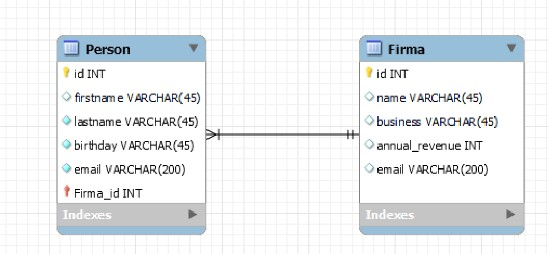
\includegraphics[width=12cm]{images/database-erd.jpg}
\end{center}

\noindent Da man nicht einfach ein Bild von einem ERD pasten kann um eine Datenbank zu erstellen haben wir ein SQL-Skript geschrieben. Dieses SQL-Skript überprüft ob es die Datenbakn schon gibt und wenn nicht erstellt es diese. Danach wählen wir die gerade erstellte Datenbank mit "USE" aus. Nun erstellen wir die beiden Tabbeln welche oben im ERD zu sehen sind. Dabür erstellen wir eine Tabelle falls diese nicht schon existiert und geben darin den Name des Attributes an, den Datentypen und Constraints an. Bei Datentypen haben wir zum einen INT gewählt was eine Ganzzahl ist. Zudem haben wir uns für VARCHAR entschieden was Text darstellt. Die Zahl in der Klammer danach steht für die länge des Textes. Bei den Constarints haben wir uns beim Primary Key für AUTOINCREMENT entschieden was soviel heisst dass bei jeder Enität die Zahl um 1 erhöht wird. NOT NULL steht dafür dass der Wert nicht Nichts sein darf, also eine Wert haben muss. Zum Schluss geben wir noch an dass die Id den Primary Key sein soll. Bei der Person Tabelle geben wir noch zusätzlich den FOREIGN KEY Constraint an und geben mit worauf sich dieser Fermdschüssel bezieht. 

\clearpage

\begin{lstlisting}[caption=SQL Script für die Datenbank]
CREATE DATABASE IF NOT EXISTS mydatabase;

USE mydatabase;

CREATE TABLE IF NOT EXISTS Firma (
  id INT NOT NULL AUTO_INCREMENT,
  name VARCHAR(255) NOT NULL,
  business VARCHAR(255) NOT NULL,
  annual_revenue INT NOT NULL,
  email VARCHAR(255) NOT NULL,
  PRIMARY KEY (id)
);

CREATE TABLE IF NOT EXISTS Person (
  id INT NOT NULL AUTO_INCREMENT,
  firstname VARCHAR(255) NOT NULL,
  lastname VARCHAR(255) NOT NULL,
  birthday DATE NOT NULL,
  email VARCHAR(255) NOT NULL,
  Firma_id INT NOT NULL,
  PRIMARY KEY (id),
  FOREIGN KEY (Firma_id) REFERENCES Firma(id)
);
\end{lstlisting}

\noindent Kommen wir zur Erstellung der RDS Instance. Dabei behandeln werden nur die Einstellungen genannt welche wir verändert haben. Falls eine Einstellungsmöglichkeit wie die Verison nicht explizit von uns genannt wird, wird davon ausgegangen dass die Standartwerte verwendet werden.
\newline
\newline
\begin{itemize}
\item \texttt{Als erstes Suchen wir in der AWS Suchleiste oben links nach "RDS" und wählen RDS aus} \\

\item \texttt{Nun wählen wir auf der Linken Seite "Datenbanken" aus} \\

\item \texttt{Danach klicken wir auf  "Datenbank erstellen"} \\

\item \texttt{Unter "Engine-Optionen" wählen wir "MySQL"} \\

\item \texttt{Unter "Vorlagen" wählen wir "Kostenloses Kontingent"} \\

\item \texttt{Unter "Einstellungen" geben wir unserer DB den Namen "database-01"} \\

\item \texttt{Unter "Einstellungen" geben wir nun unser gewünschtes Passwort ein, nähmlich "Sml12345" und bestätigen dieses} \\

\item \texttt{Unter "Anbindung " beim Punkt "Öffentlicher Zugriff" wählen wir "Ja" damit wir auch von ausserhalb des VPC auf unsere DB zugreifen können} \\

\item \texttt{Zum Schluss der Erstellung klicken wir nun "Datenbank erstellen" und warten darauf dass die DB gestartet ist } \\

\item \texttt{Nun wählen wir auf der Linken Seite "Datenbanken" aus} \\

\item \texttt{Danach klicken wir auf unsere DB und kopieren unter "Endpunkt und Port" den Endpunkt} \\

\item \texttt{Nun klicken wir oben rechts, links von der Glocke auf das console-Icon} \\

\item \texttt{Um uns mit der DB zu verbinden geben wir folgenden Befehl ein: "mysql -h <endpoint> -u admin -p". <endpoint> wird jedoch durch die Addresse des Endpoint welche wir vorher kopiert haben ersetzt.} \\

\item \texttt{Nun geben wir noch unser Passwort ein, was in unserem Fall "Sml12345" ist} \\

\item \texttt{Jetzt sind wir mit der DB verbunden, da wir jedoch noch keine Tabellen haben kopieren wir das SQL-Skript von oben, fügen es ein und bestätigen dass wir dies auch wirklich wollen und drücken ENTER} \\

\item \texttt{Um zu überprüfen ob es geklappt hat können wir folgenden bBefehl eingeben und es sollten uns unsere 2 Tabellen angezeigt werden: "show tables;"} \\

\end{itemize}

\noindent Zudem kann man sich z.B. mit MySqlWorkbench auf die DB verbinden und änderungen vornehmen.

\clearpage

\section{S3}

\subsection{Beschreibung}
Mit Amazon Simple Storage Service, kurz S3, möchten wir eine Nextcloud erstellen. Da das S3 nur ein Speicher ist benötigen wir dazu noch eine EC2 Instance welche das GUI der Nextcloud zu verfügung stellt und über welches wir auf unseren S3 Bucket zugreifen können und auf diesem Daten verwalten können.

\subsection{Installation}

\noindent Um nun das Ganze zu erstellen, loggen wir uns als erstes im Learner Lab ein und starten dieses. Nun besuchen wir die aws console.

\begin{itemize}
\item \texttt{Als erstes suchen wir nun in der Suchleiste nach "EC2" und wählen diesen Dienst aus.} \\

\item \texttt{Klicke rechts oben auf den "Instance Starten"-Button.} \\

\item \texttt{Gib unter "Name und Tags" den Namen "next-cloud-01" } \\

\item \texttt{Unter "Anwendungs- und Betriebssystemabbilder" drückst du auf "Weitere AMI's durchsuchen"} \\

\item \texttt{Suche in der Suchleiste nach "Ubunut Server" und wähle diesen aus:
} \\

\begin{center}
    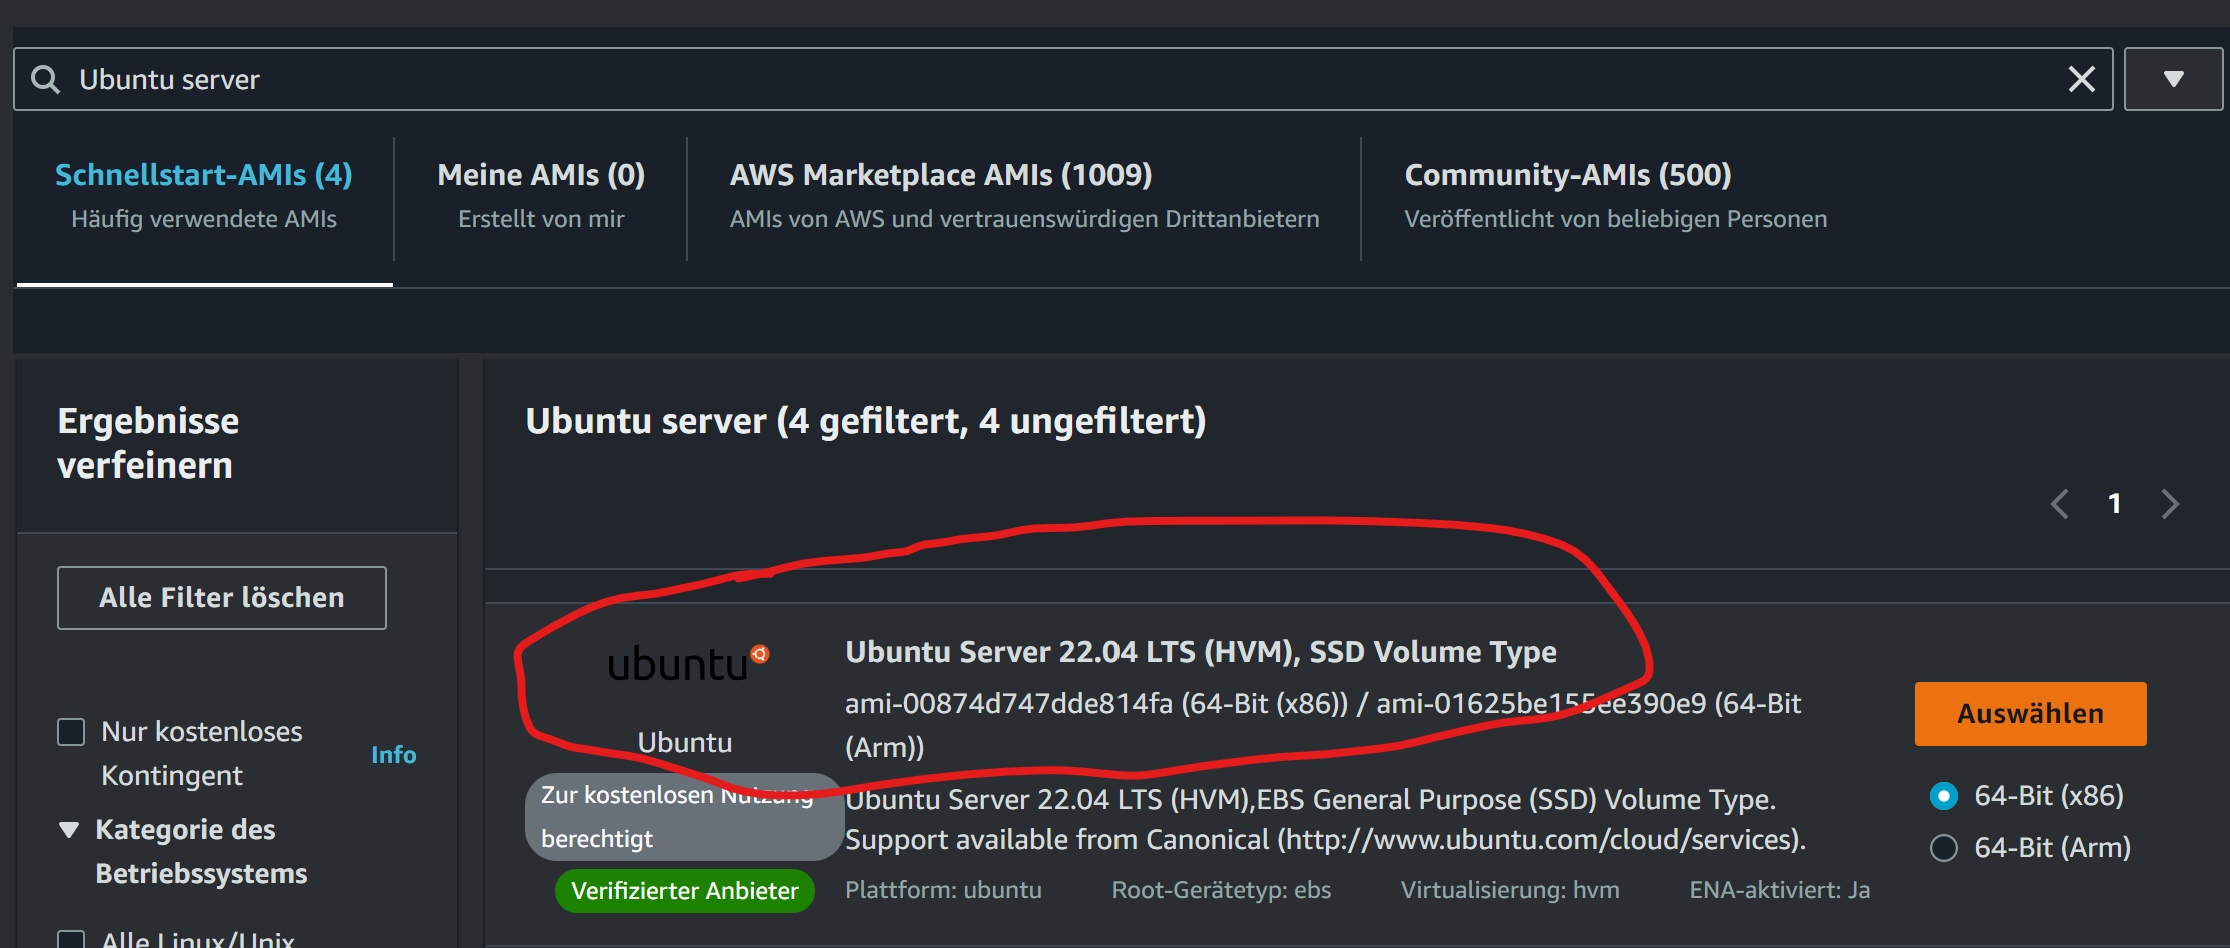
\includegraphics[width=13cm]{images/nextcloud_1.png}
\end{center}

\clearpage

\item \texttt{Unter "Instance-Typ" wählst du "t3.micro" aus.} \\

\item \texttt{Beim Schlüsselpaar wählst du dir ein Schlüsselpaar deiner Wahl aus oder erstellst eines.} \\

\item \texttt{Unter den "Netzwerkeinstellungen" wählst du folgende Konfiguration aus: 
} \\
\begin{center}
    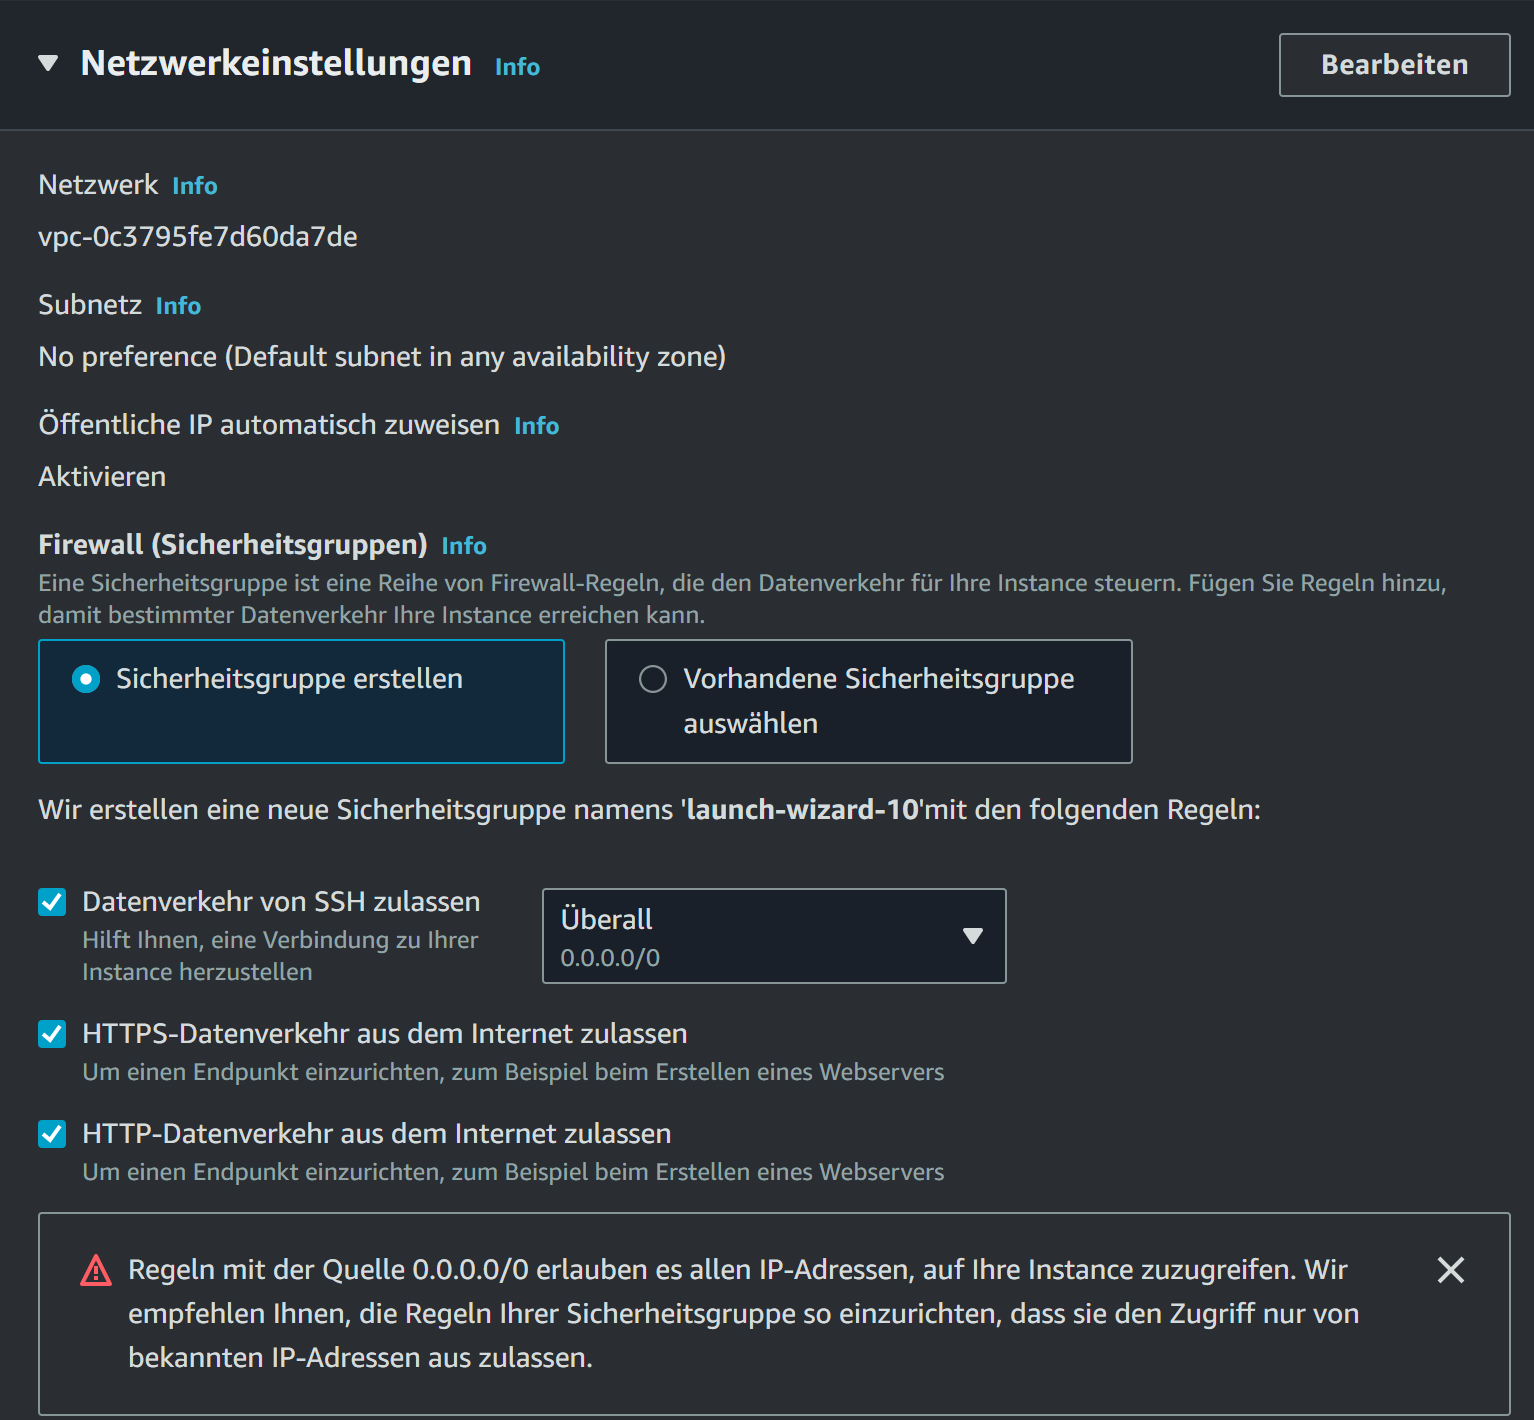
\includegraphics[width=13cm]{images/nextcloud_2.png}
\end{center}

\item \texttt{Alle anderen Einstellungen kannst du so lassen wie sie sind. Klicke nun auf "Instance erstellen"} \\

\clearpage

\item \texttt{Kehre nun auf die Übersicht deiner Instances zurück. Nun solltest du deine neue Instance sehen.} \\

\item \texttt{Klicke auf der Linken Seite auf "Elastic Ip's" und danach auf "Elastic IP Adresse zuweisen"} \\

\item \texttt{Scrolle nach unten und drücke "Zuweisen".} \\

\item \texttt{Wähle nun deine Elastic IP aus und drücke "Elastic IP Adresse zuordnen", wähle deine Instance aus und drücke "zuordnen"} \\

\item \texttt{Kehre nun auf die Übersicht deiner Instances zurück. Nun solltest du deine neue Instance sehen.} \\

\item \texttt{Wenn deine EC2 Instance läuft klicke auf ihre Id und danach auf "Verbinden".} \\

\item \texttt{Wähle "EC2 Instance Verbindung" aus und klicke "Verbinden":
} \\

\begin{center}
    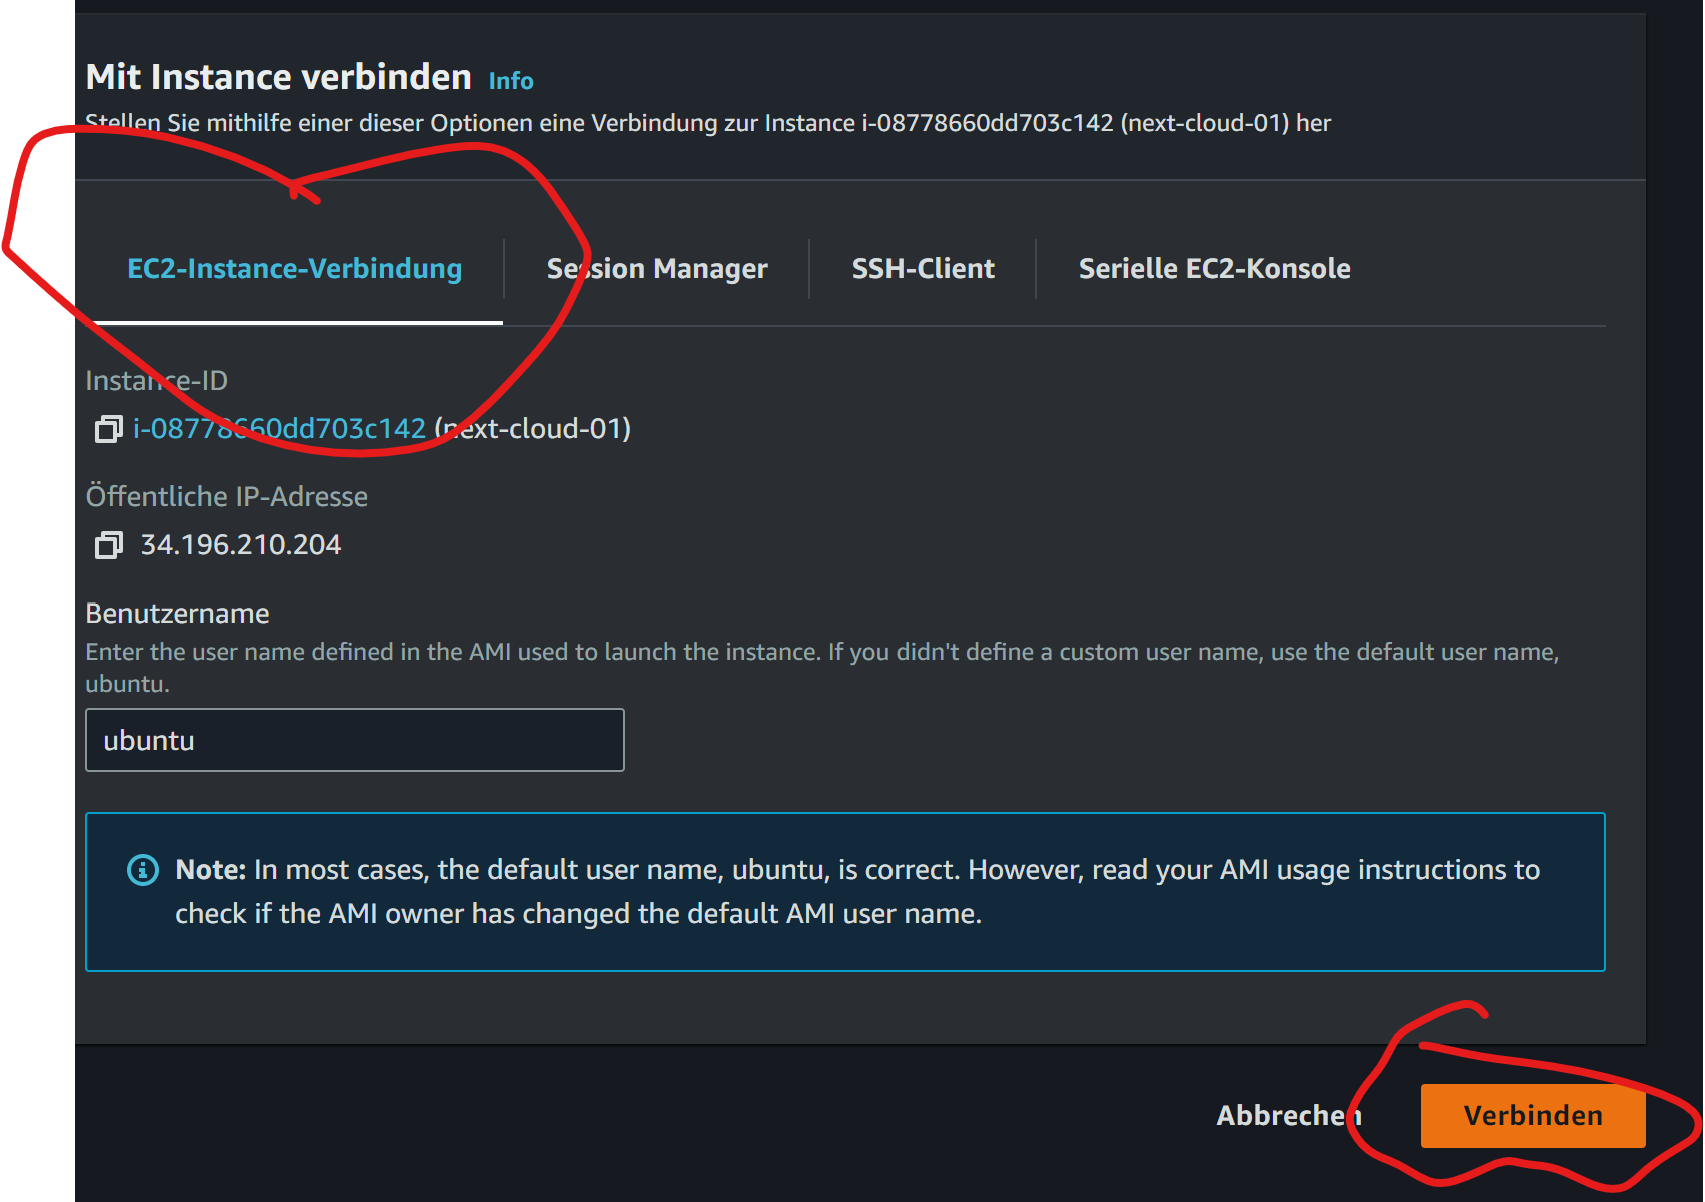
\includegraphics[width=13cm]{images/nextcloud_3.png}
\end{center}

\item \texttt{Nun solltest du dich in einem Terminal im Browser befinden. Instaliere die Nextcloud Software mit folgendem Command "sudo snap install nextcloud"} \\

\item \texttt{Gebe nun folgenden Command ein: "sudo nextcloud.manual-install <adminusername> <adminpassword>". adminusername und adminpassword kannst du selbst wählen, jedoch merke dir was du gewählt hast.} \\

\item \texttt{Als nächstes nutzen wir folgenden Command um Nextcloud zu sagen von welcher IP wir zugreifen möchten: "sudo nextcloud.occ \\config:system:set trusted\_domains 1 --value=<dns-domain>". Ersetze "dns-domain" durch deine Elastic IP.} \\

\item \texttt{Zum Schuss nutzen wir noch diesen Command: "sudo snap set nextcloud nextcloud.cron-interval=10m".} \\

\item \texttt{Nun kannst du mit http über deine Elastic IP im Brower auf deine Nextcloud verbinden. Dies sollte etwa so aussehen: 
} \\

\begin{center}
    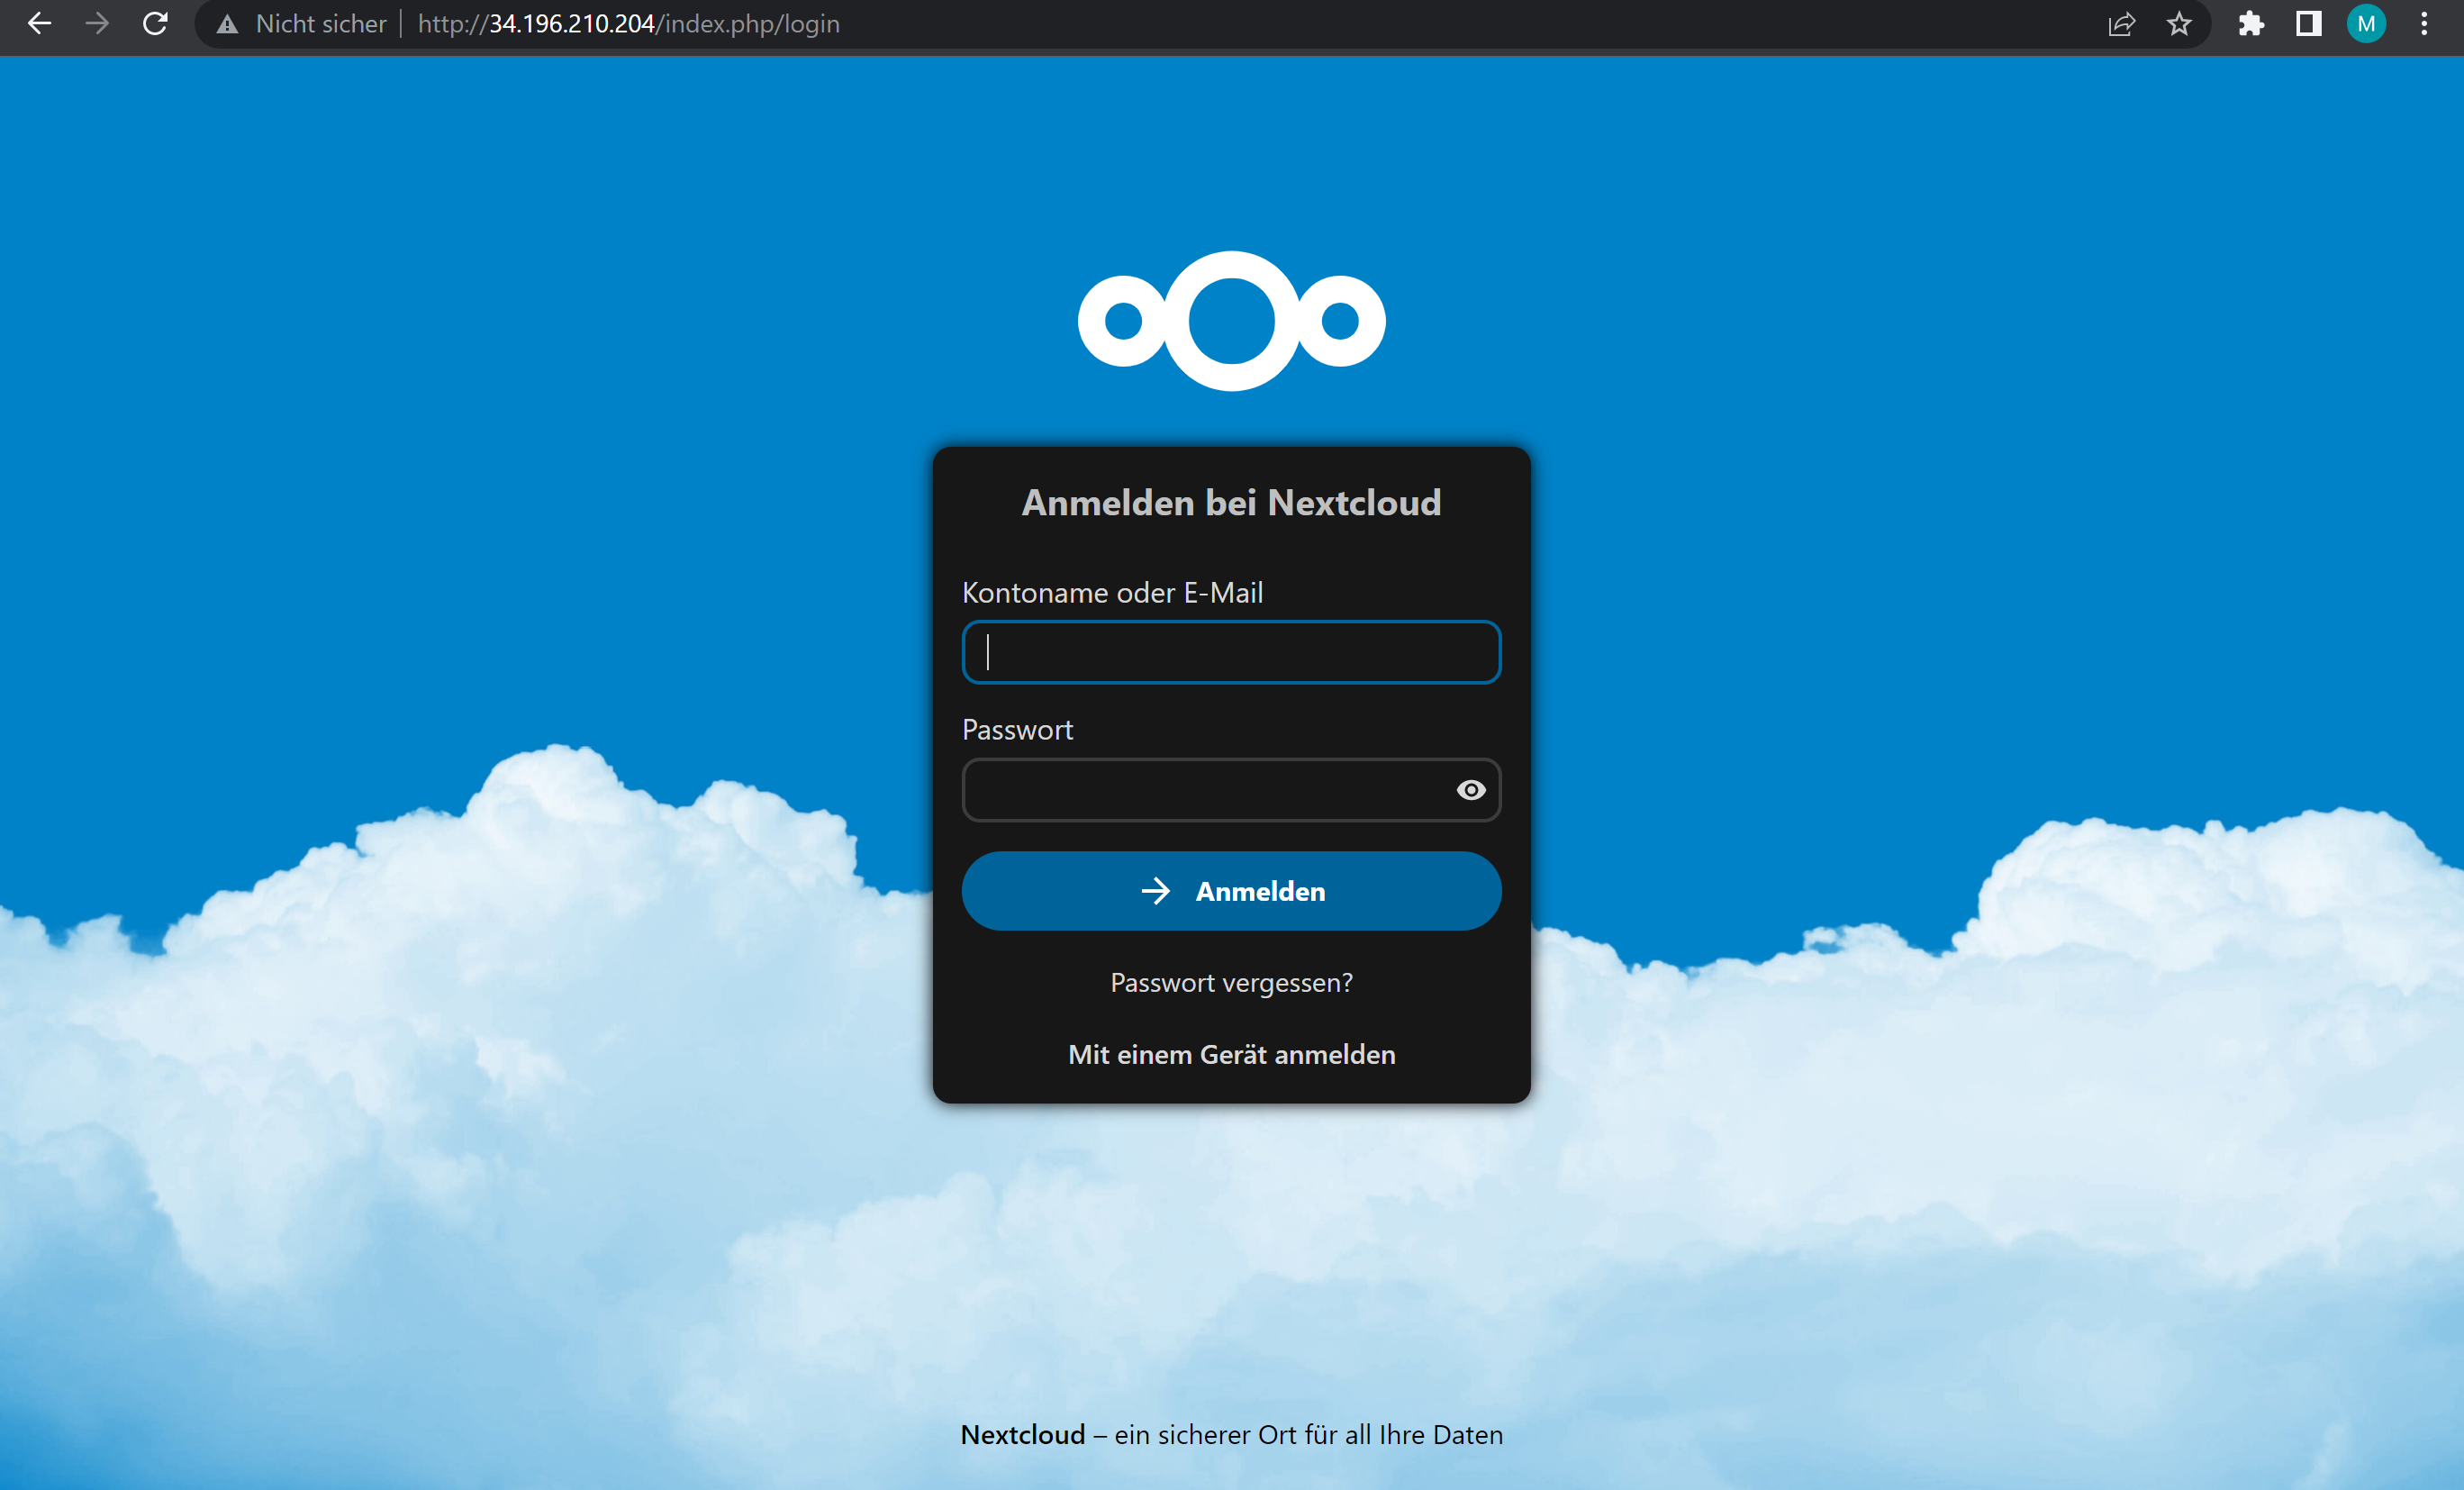
\includegraphics[width=13cm]{images/nextcloud_4.png}
\end{center}

\clearpage

\item \texttt{Nun kannst du dich mit den Daten anmelden welche du vorher im Command ersetzt hast, in unserem Fall als Name "admin" und als Passwort "sml12345".} \\

\item \texttt{Drücke nun oben Rechts auf deinen Account und wähle "Apps". Danach "Deaktivierte Apps". Aktiviere nun "External storage support".} \\

\item \texttt{Wechsle zurück in deine AWS Console und suche in der Suchleiste nach "S3" und wähle diesen Dienst aus.} \\

\item \texttt{Clicke nun auf "Bucket erstellen" und gib diesem einen Einzigartigen Namen.} \\

\item \texttt{Die andere Einstellungen kannst du lassen wie sie sind. Scrolle nach unten und drücke "Bucket erstellen."} \\

\item \texttt{In der Nextcloud kannst du nun nochmals auf dein Profil klicken und danach "Administratoreinstellungen" und danach "Externer Speicher"} \\

\item \texttt{Nehme dort folgende Konfiguration vor. Wobei du "your-bucket-name" durch den vorher gewählten Bucketname ersetzt.
} \\

\begin{center}
    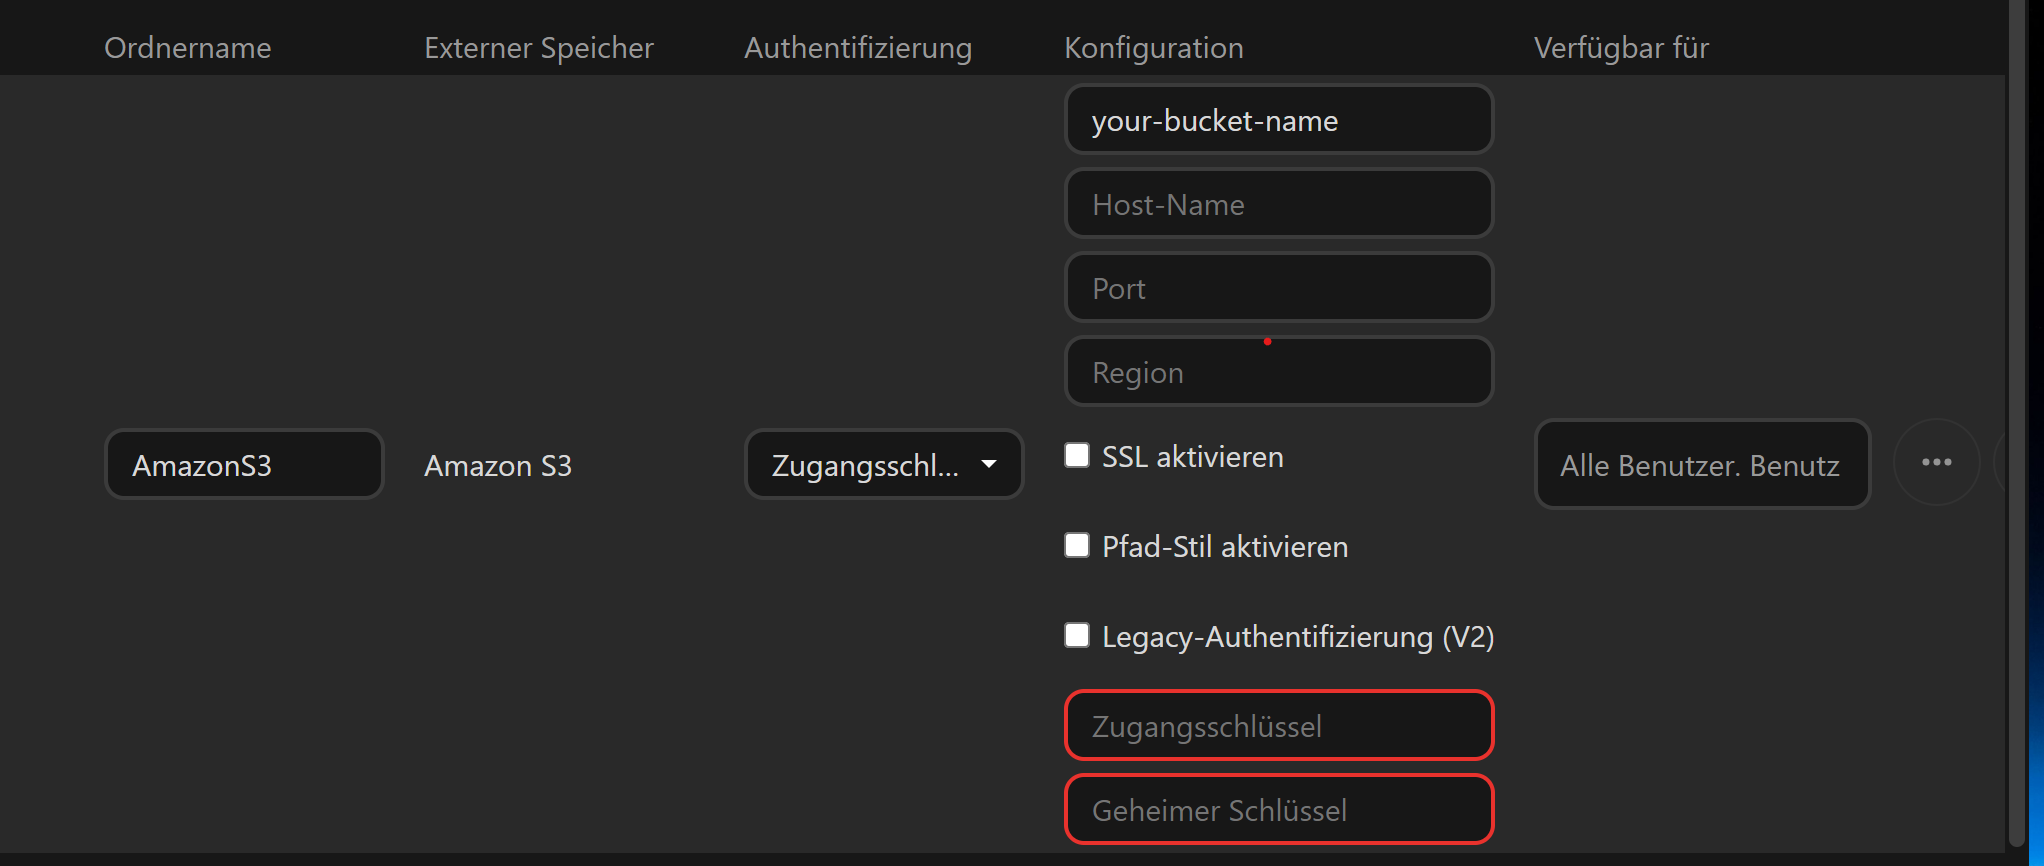
\includegraphics[width=13cm]{images/nextcloud_5.png}
\end{center}

\clearpage

\item \texttt{Den Zugangsschlüssel und geheimen Zugangsschlüssel findest du im Learner Lab:
} \\

\begin{center}
    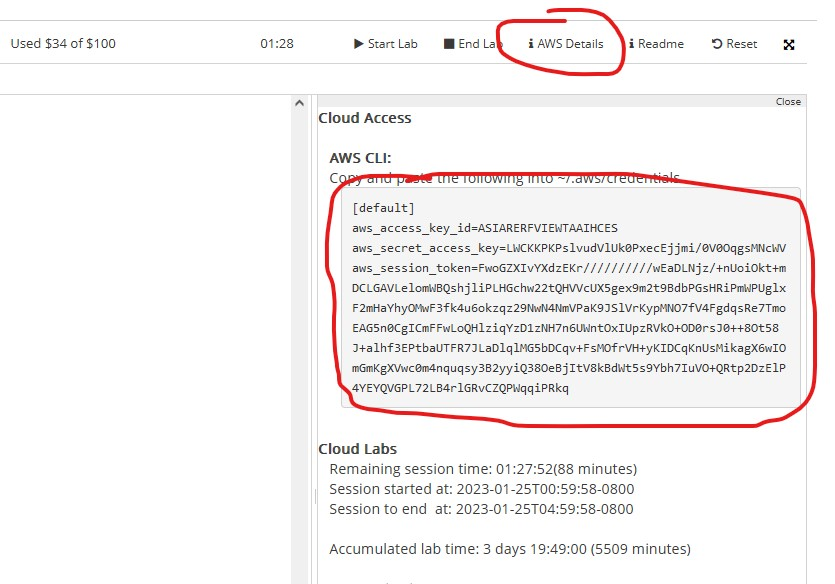
\includegraphics[width=13cm]{images/wordpress_2.jpg}
\end{center}

\end{itemize}

\subsection{Verfügbarkeit}

\noindent In Bezug auf die Verfügbarkeit wurde die Nextcloud-Instanz auf einer EC2-Instanz in der Zone US-EAST1 bereitgestellt. Es wurde nur ein AWS-Account verwendet. Obwohl die Verwendung mehrerer Zonen und Accounts die Verfügbarkeit weiter erhöhen kann, gewährleistet die Verwendung einer Zone und eines Accounts immer noch eine hohe Verfügbarkeit der Nextcloud-Instanz.

\subsection{Datensicherheit}

\noindent In Bezug auf die Datensicherheit werden die Daten der Nextcloud auf einem S3-Storage gespeichert. Dieser bietet eine hohe Redundanz und Verfügbarkeit der Daten, um sicherzustellen, dass die Daten auch im Falle eines Ausfalls des Storage-Systems weiterhin verfügbar sind. Leider haben wir keine Wiederherstellung eingerichtet. Diese Möglichkeit besteht jedoch durch die Verwendung von S3, da es automatisch Backups und Wiederherstellungsmöglichkeiten für Daten bereitstellt.

\subsection{Kostenanlyse}
Wir haben für die Kostenanalyse den AWS Pricing Calculator verwendet. Wir gehen davon aus dass wir eine EC2 von der Grösse t3.micro, eine Elastic Ip und einen S3 Bucket verwenden. Der S3 Bucket hat eine Grösse 20 GB. Andere Services werden für die Nextcloud nicht verwendet.
\newline
Vorabkosten entstehen keine für dieses kleine Projekt. Die Elastic Ip ist kostenlos da wir nur eine für die EC2 Instance verwenden. Die Nextcloud Software welche wir nutzen ist auch kostenlos. Für die EC2 Instance bezahlen wir 7.59 Dollar pro Monat. Das S3 Bucket ist erstaunlich Günstig mit einem Preis von 49 Mill im Monat. Zusammen mach das 8.08 Dollar im Monat und 96.98 Dollar im Jahr.

\clearpage

\section{Amazon Elastic Container Service }

\subsection{Beschreibung}

\noindent Mit Amazon Elastic Container Service, kurz ECS, wollen wir einen Wordpress Blog mithilfe von EC2 Instances hosten. Da jedoch sind fast alle in öffentlichen Foren wie StackOverFlow, in Blogposts oder in YT-Tutorials der Meinung dass man das Ganze am Besten mit Fargate anstatt mit EC2 umsetzt. Deshalb benutzen wir in unserem Projekt für unseren Wordpress-Blog die AWS Dienste ECS, ECR, und Fargate.
\newline 

\subsection{Installation}

\noindent Um nun das Ganze zu erstellen, loggen wir uns als erstes im Learner Lab ein und starten dieses. Nun besuchen wir die aws console.

\begin{itemize}
\item \texttt{Als erstes suchen wir nun in der Suchleiste nach "ECR" und wählen diesen Dienst aus.} \\

\item \texttt{Auf der Rechten Seite klicken wir nun auf "Repository erstellen"} \\

\clearpage

\item \texttt{Nun nehmen wir folgende Konfiguration vor und drücken auf "Repository erstellen":
} \\

\begin{center}
    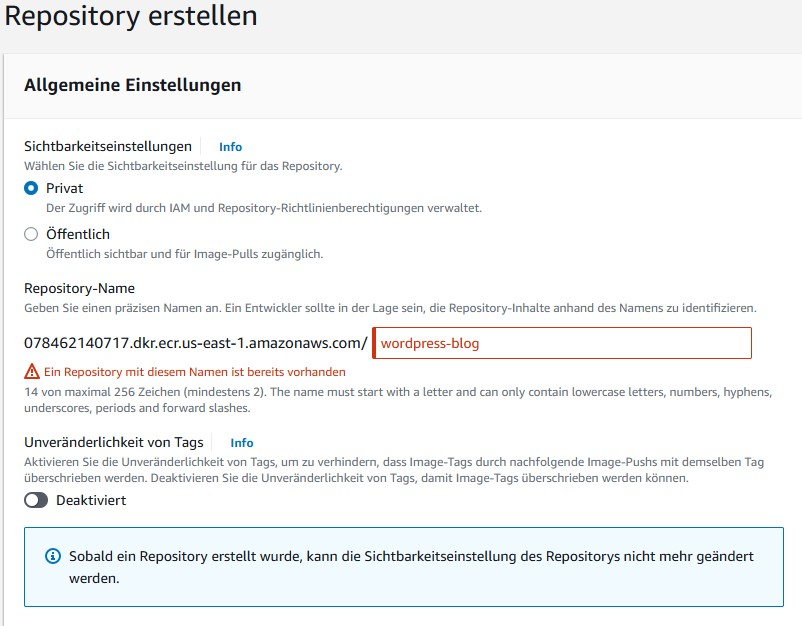
\includegraphics[width=13cm]{images/wordpress_1.jpg}
\end{center}

\item \texttt{Stelle sicher dass du den AWS CLI instaliert hast, falls nicht downloade diesen unter "https://docs.aws.amazon.com/cli/latest/userguide/ getting-started-install.html".} \\

\clearpage

\item \texttt{Stelle nun sicher dass du den die credentials vom Learner Lab ins "credentials"-File in deinem Userhome im ".aws"-Ornder kopierst. Die Credentials findest du im Learner Lab, dort wo du auch dieses startest unter "AWS Details": 
} \\

\begin{center}
    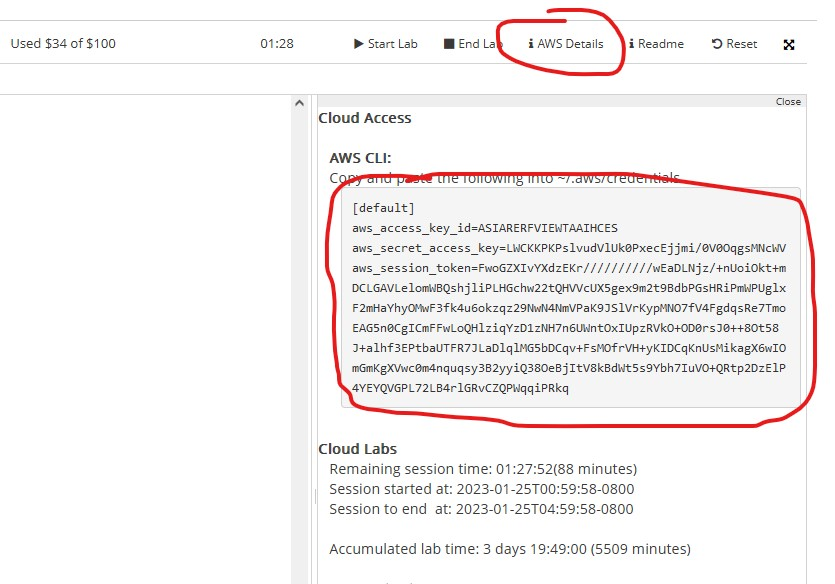
\includegraphics[width=13cm]{images/wordpress_2.jpg}
\end{center}

\item \texttt{Öffne eine Lokale Konsole und gebe folgenden befehl ein "aws ecr get-login-password --region us-east-1 | docker login --username AWS --password-stdin {ACCOUNTID}.dkr.ecr.us-east-1.amazonaws.com" Für {ACCOUNTID} gibst du deine Account Id ein welche du unter anderm in deinem Profil nachscheun kannst.} \\

\item \texttt{Als nächstes nutzen wir folgenden Command um das offizielle Dockerimage von Dockerhub zu ziehen: "docker pull wordpress"} \\

\item \texttt{Nun möchten wir dieses Image zu ECR pushen. Dies können wir mit diesem Command "docker tag wordpress {ACCOUNTID}.dkr.ecr.us-east-1.amazonaws. com/sample-wordpress:latest" gefolgt von diesem "docker push {ACCOUNTID}. dkr.ecr.us-east-1.amazonaws.com/sample-wordpress:latest" erreichen. Auch hier wieder {ACCOUNTID} durch deine eigene Account-Id ersetzten.} \\

\item \texttt{Nun kannst du in deinem ECR-Repository, welches wir erstellt haben das Image sehen. Kopiere davon die URL da wir diese später benötigen: 
} \\

\begin{center}
    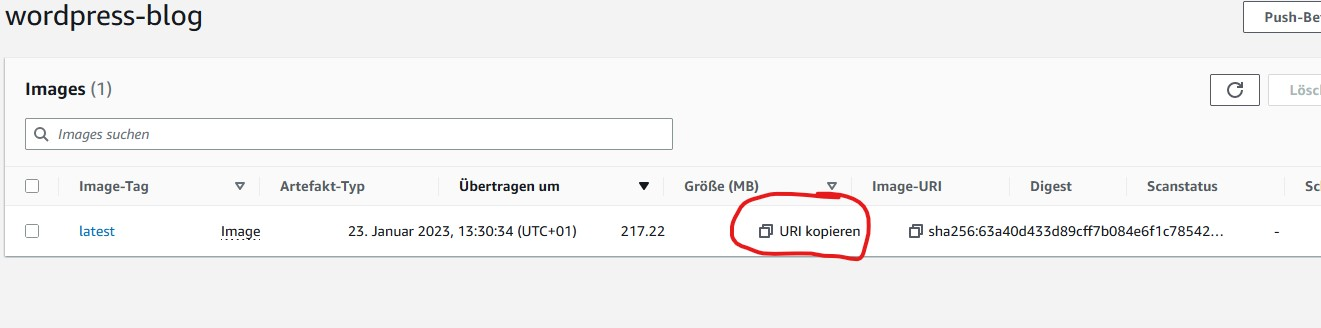
\includegraphics[width=14cm]{images/wordpress_3.jpg}
\end{center}

\item \texttt{Suche nun in der Suchleiste oben links nach "ECS" und wähle diesen Dienst aus.} \\

\item \texttt{Falls es oben in der Mitte keinen Button mit "Erste Schritte hat, dann toggle den Toggle-Button oben links welcher mit "Neue ECS-Umgebung" beschriftet ist:
} \\

\begin{center}
    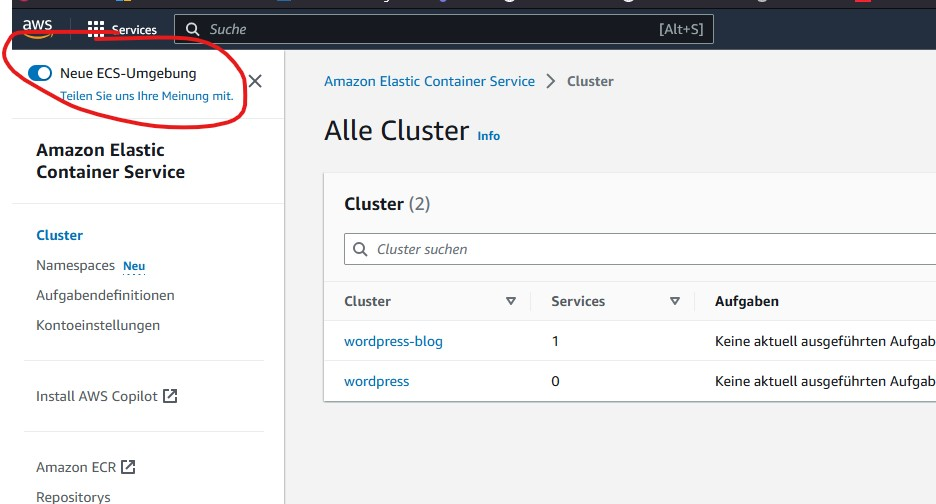
\includegraphics[width=13cm]{images/wordpress_4.jpg}
\end{center}

\item \texttt{Klicke nun auf "Erste Schritte und wähle "custom" aus und klicke auf "konfigurieren".} \\

\item \texttt{Gebe nun folgende Konfiguran an wobei du {IMAGE URL} durch die vorher kopierte Image URL ersetzt und drücke unten rechts auf aktualisieren: 
} \\

\begin{center}
    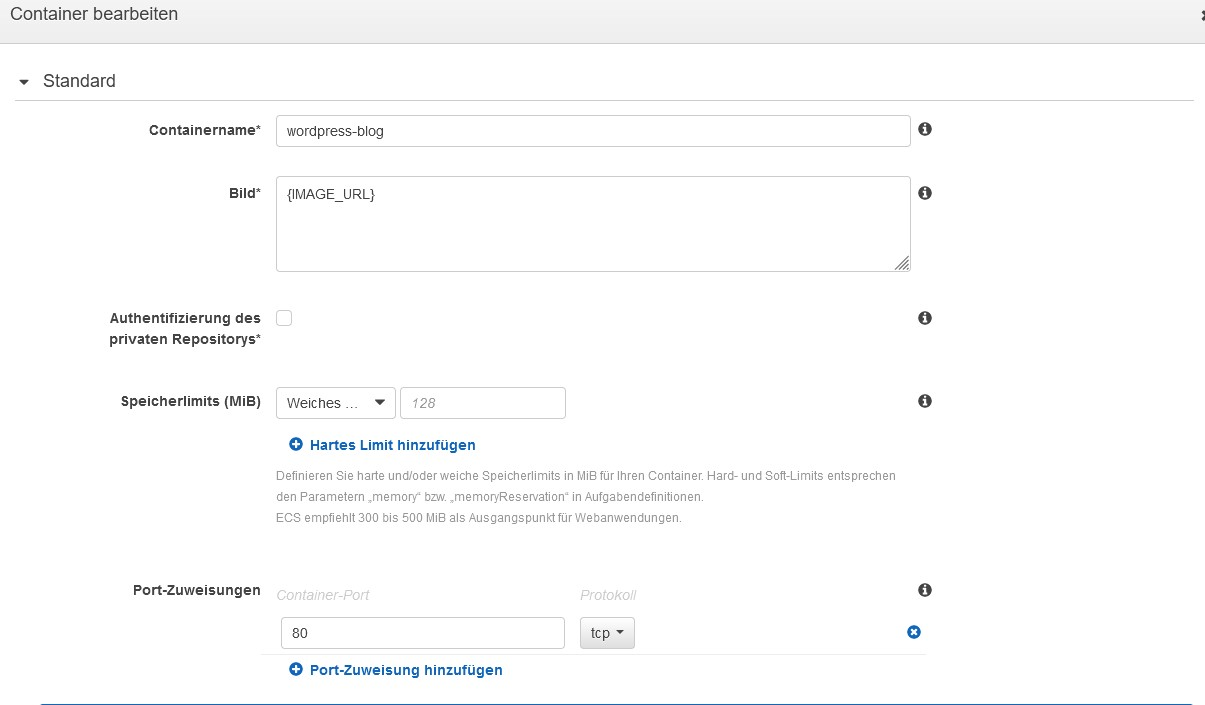
\includegraphics[width=13cm]{images/wordpress_5.jpg}
\end{center}

\item \texttt{Unter "Aufgabendefinition" klickst du auf bearbeiten und änderst den Namen der Aufgabendefinition zu "wordpress-blog" und setzte die "Aufgabenausführungsrolle" zu "LabRole" und speichere und drücke "weiter".} \\

\item \texttt{Klicke nun auf weiter.} \\

\item \texttt{Wähle unter "Load Balancer" Application Load Balancer aus und klicke "weiter" an.} \\

\item \texttt{Jetzt kannst du dir noch einen Cluster-Namen aussuchen eun weiter klicken} \\

\clearpage

\item \texttt{Jetzt wird dir die Gesamte konfiguration angezeigt. Scroll nach unten und erstelle den Cluster. Dies solle nun etwa so aussehen: 
} \\

\begin{center}
    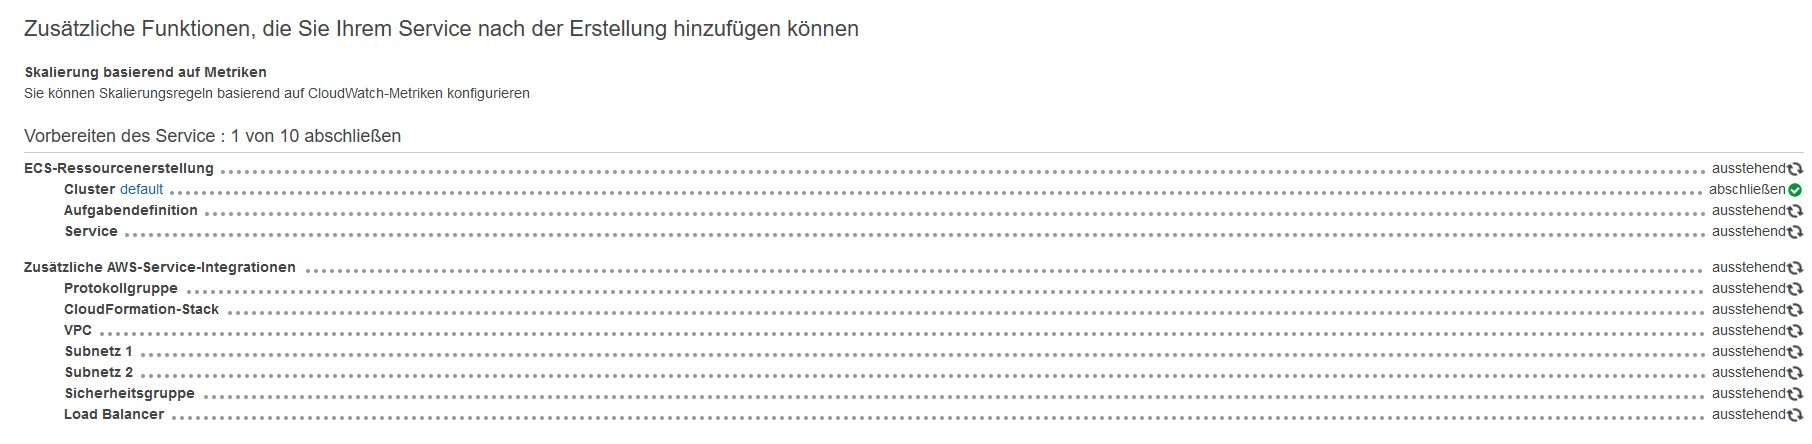
\includegraphics[width=13cm]{images/wordpress_6.jpg}
\end{center}

\item \texttt{Nun wollen wir noch wissen wie wir überhaupt daraus zugreiffen können. Dafür suchst du in der Suchleiste oben rechts nach EC2 und wählst diesen Dienst aus.} \\

\item \texttt{Auf der Linken Seite wählst du nun "Load Balancer" aus: 
} \\

\begin{center}
    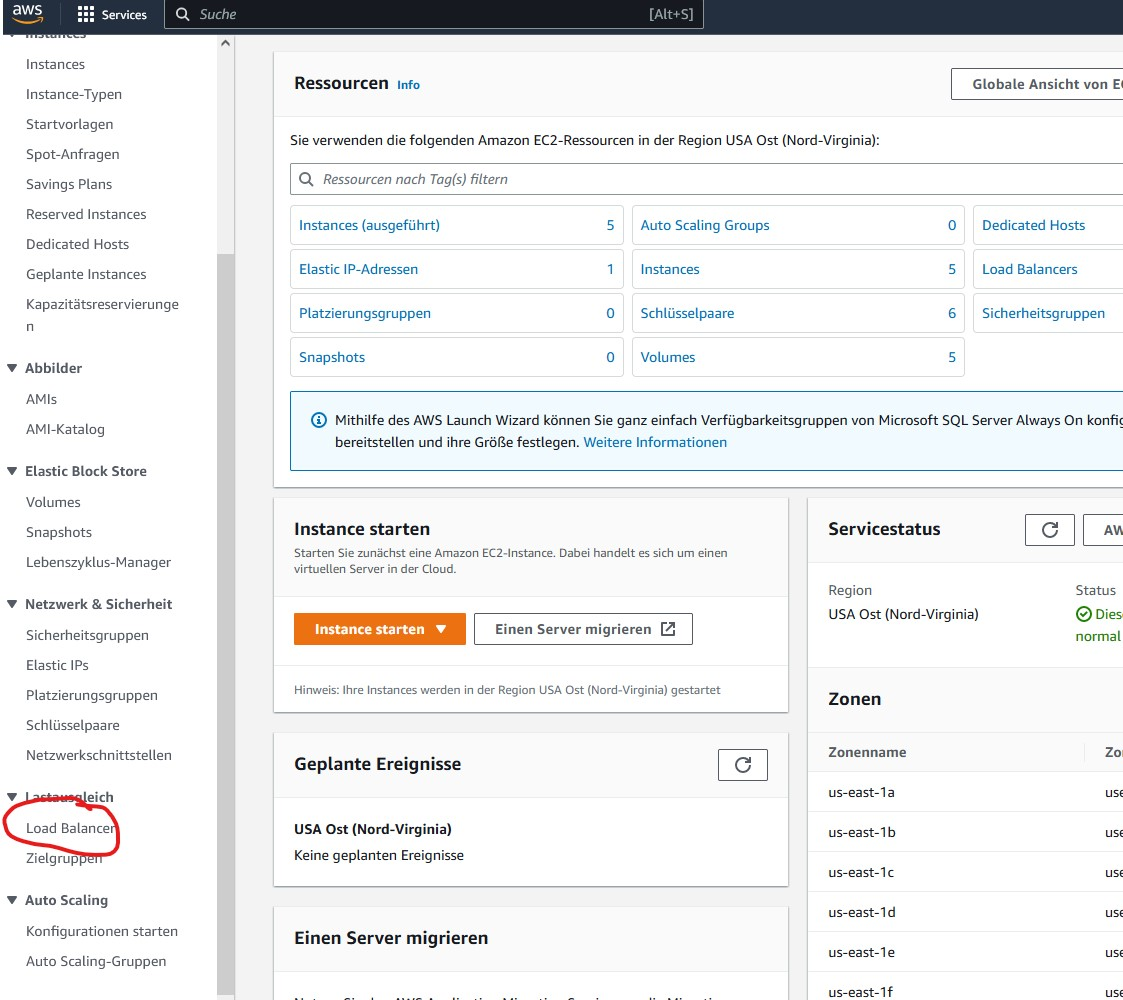
\includegraphics[width=11cm]{images/wordpress_7.jpg}
\end{center}

\item \texttt{Nun klickst du auf den Namen deines Load Balancers: 
} \\

\begin{center}
    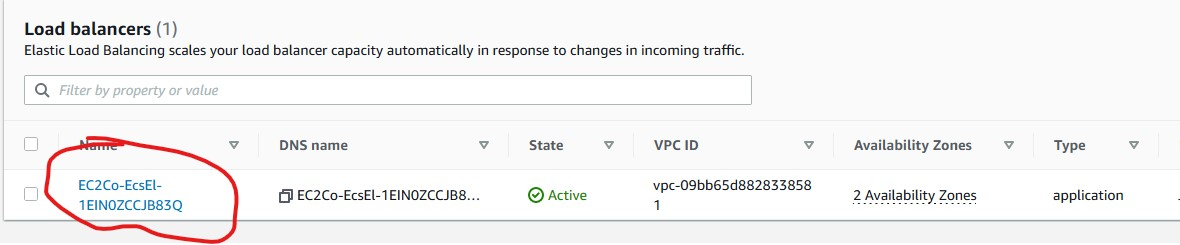
\includegraphics[width=13cm]{images/wordpress_8.jpg}
\end{center}

\item \texttt{Der DNS Name ist nun die URL mit welcher du auf deine Wordpressseite zugreiffen kannst: 
} \\

\begin{center}
    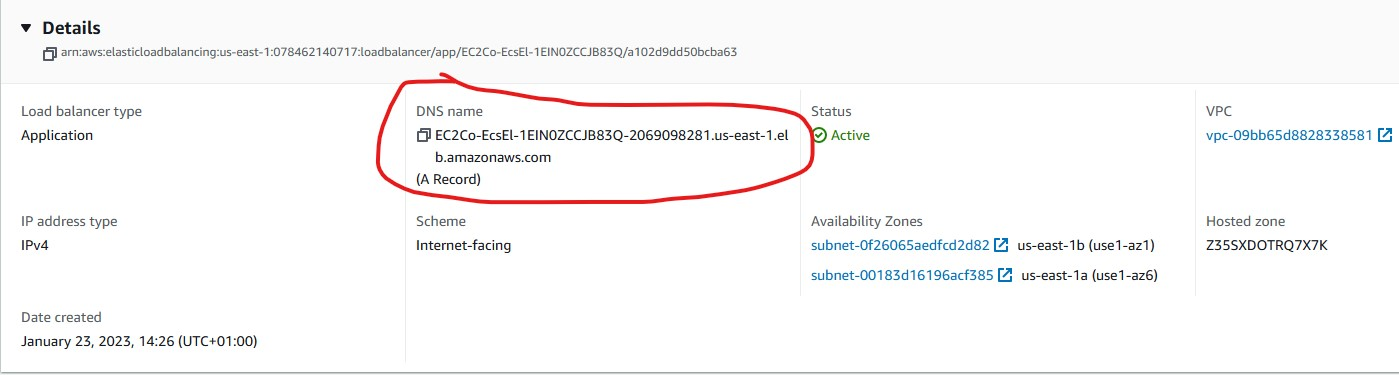
\includegraphics[width=13cm]{images/wordpress_9.jpg}
\end{center}

\item \texttt{Wenn wir nun auf die Seite zugreiffen sollte es folgendermassen aussehen: 
} \\

\begin{center}
    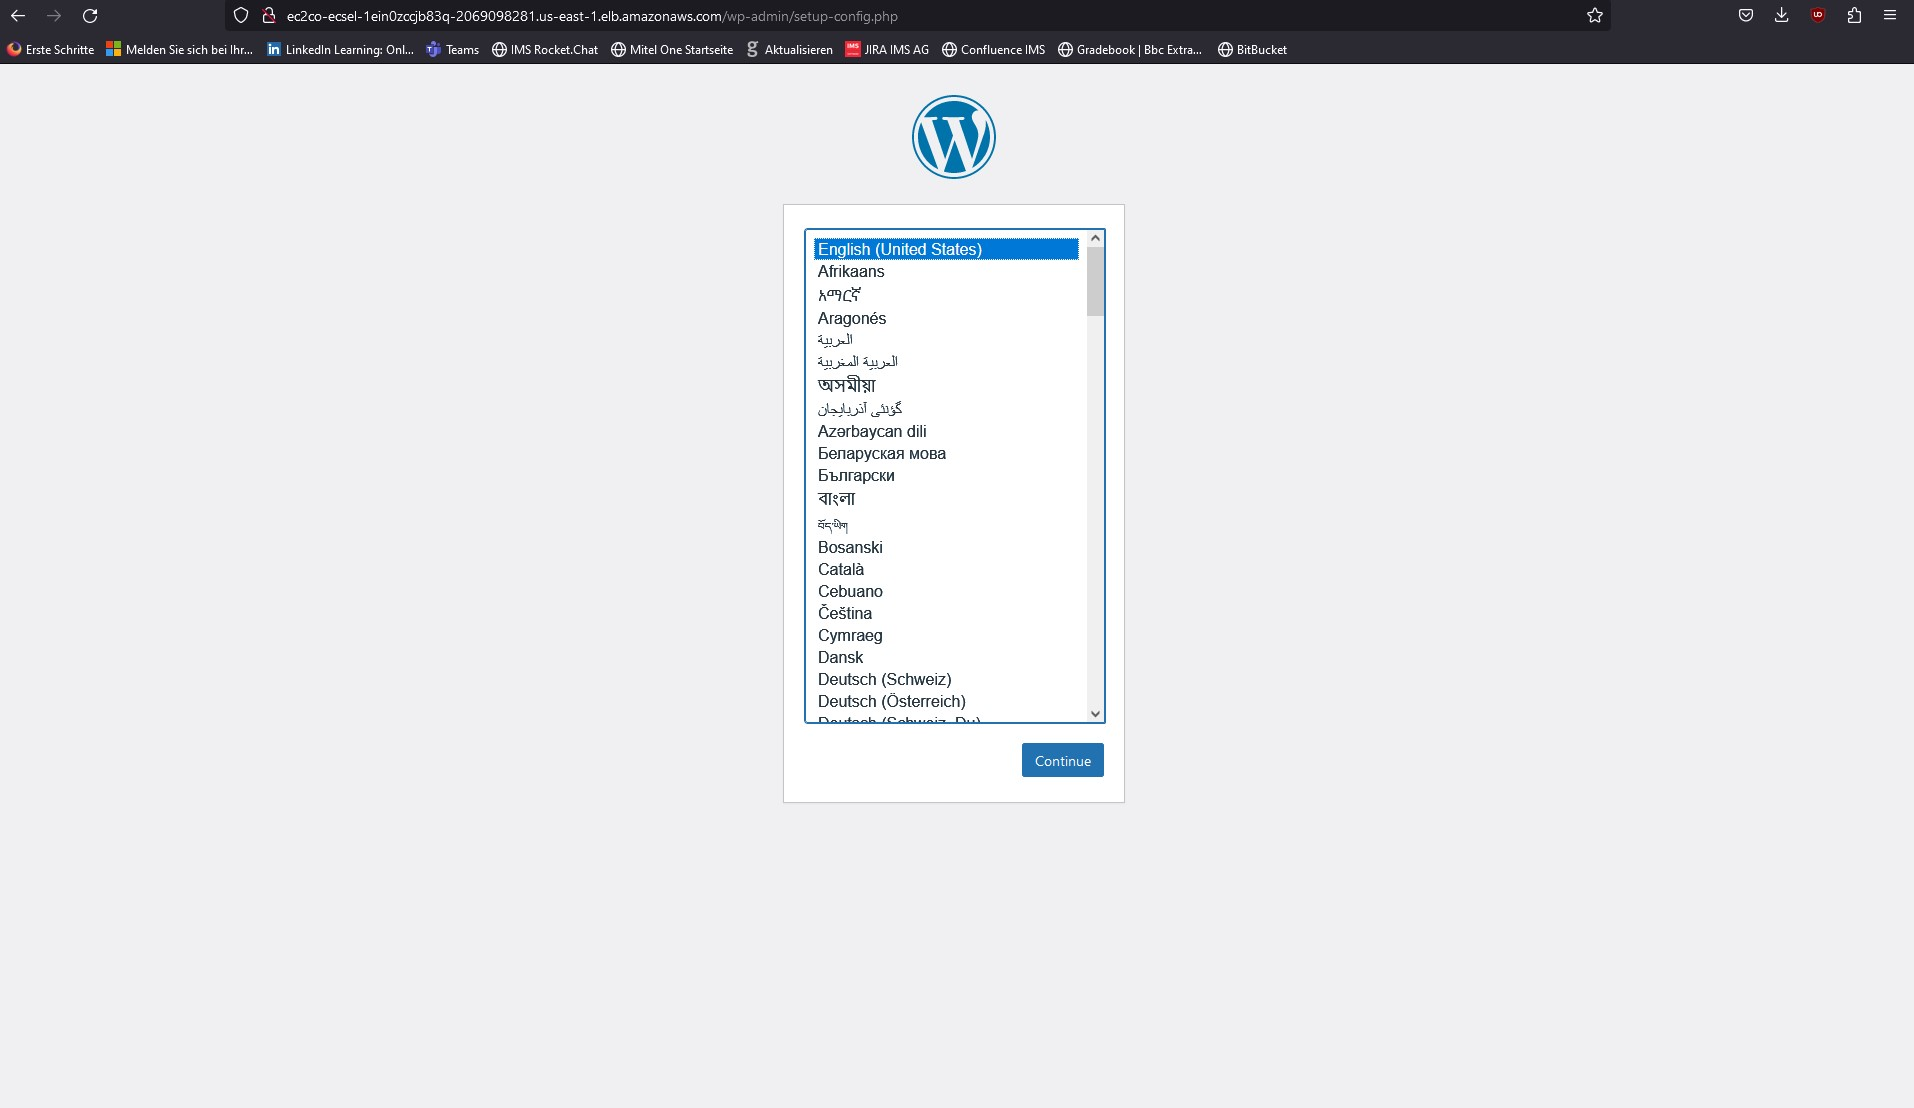
\includegraphics[width=12cm]{images/wordpress_10.jpg}
\end{center}

\end{itemize}

\subsection{Verfügbarkeit}
Der Cluster und die dazugehörigen Komponenten sind nur in der Region us-east-1 verfügbar. Dies schliesst jedoch nicht aus dass man ihn von der ganzen Welt aus anschauen kann, die Latenzen sind einfach höher. Zudem kann man nur Änderungen an den Komponenten mit dem in der Einleitung genannten Account vornehmen.

\subsection{Datensicherheit}
Bezüglich der Datensicherheit fallen keine grosse Risiken auf. Den der Cluster auf welchem der Blog läuft wurde mit einem Wordpress-Image aufgesetzt welches man jederzeit auf Dockerhub wieder bekommen kann. Der Blog selbst würde auf einem RDS System laufen welches selbst eine Backup-Funktion bietet was einen Datenverlust fast zu 100 Prozent ausschliesst.

\subsection{Kostenanlyse}
Wir haben unsere Kostenanalyse mit dem AWS Pricing Calculater für die Region us-east-1 also North-Virginia erstellt. Dabei haben wir die Services ECS, Fargate und RDS eingebunden. Du wirst dich warscheinlich fragen "RDS?". Ja, wenn wir wirklich einen Blog hosten möchten brauchen wir noch eine DB. Da diese jedoch nicht zu unserem Service gehört haben wir diese ausgelassen denn wir haben RDS schon verwenden und haben auch nicht genügend Zeit für alles da die Nextcloud schon extrem viel Zeit in anspruch genommen hat. Für die DB haben wir angenommen dass wir eine MySQL DB mit 10 GB storage und nochmal 10 GB für ein Backup nutzen damit wir unsere Daten sicher können. Bei ECS und Fargate haben wir mit Durchschnittlich 10 Connections pro Tag gerechnet.
\newline
\newline
Somit sind wir auf folgende Kosten gekommen. Pro Monat würden wir für ECS 38 Mill, für Fargate 39 Mill und für RDS 28.01 Dollar bezahlen. Zusammen mach das 28.78 Dollar pro Monat. Im Jahr sind das 345.42 Dollar.

\begin{center}
    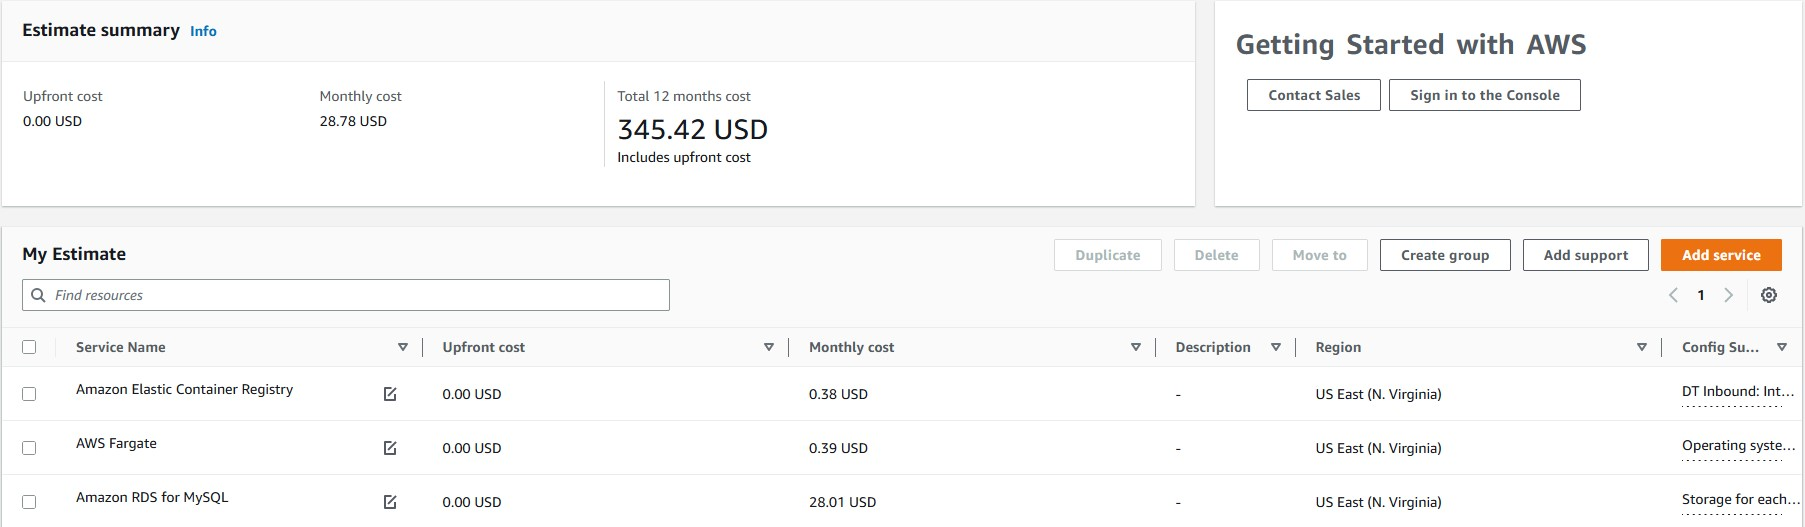
\includegraphics[width=12cm]{images/wordpress_11.jpg}
\end{center}

\end{document}
